\documentclass[12pt,a4paper]{article}
%\usepackage[allfiguresdraft]{draftfigure}
%\newcommand{\pdfextension}{pdf}
%\newcommand{\pngextension}{png}
\usepackage{cite}
\usepackage{natbib}
\usepackage{breakcites}
\usepackage[normalem]{ulem}
\usepackage{comment}
\usepackage[font=footnotesize,labelfont=bf]{caption}
\let\rho=\varrho

\def\fref#1{Fig.~\ref{#1}}
\def\tabref#1{Table~\ref{#1}}
\def\cref#1{Condition~\ref{#1}}
\def\Cref#1{Corollary~\ref{#1}}
\def\eref#1{(\ref{#1})}
\def\sref#1{\textsection\ref{#1}}
\def\lref#1{Lemma~\ref{#1}}
\def\rref#1{Remark~\ref{#1}}
\def\tref#1{Theorem~\ref{#1}}
\def\dref#1{Definition~\ref{#1}}
\def\pref#1{Proposition~\ref{#1}}
\def\aref#1{Assumption~\ref{#1}}
\def\qref#1{Subsection~\ref{#1}}

\def\dref#1{Definition~\ref{#1}}
\def\myundefined#1{\special{ps: 1 0 0 setrgbcolor}{what is #1?}%
	\special{ps: 0 0 0 setrgbcolor}}
\newenvironment{myitem}
{\begin{itemize}
  \setlength{\itemsep}{1pt}
  \setlength{\parskip}{0pt}
  \setlength{\parsep}{0pt}}
{\end{itemize}}

\newenvironment{myenum}
{\begin{enumerate}
  \setlength{\itemsep}{1pt}
  \setlength{\parskip}{0pt}
  \setlength{\parsep}{0pt}}
{\end{enumerate}}

%\usepackage{sub_JP}
%\usepackage{fancyhdr}
%\pagestyle{fancy}
\usepackage{amsmath}
\usepackage{amsfonts}
\usepackage{graphicx}
%\usepackage{makeidx}
\usepackage{times}
\usepackage{amsthm}
\usepackage{ amssymb }
\usepackage{color}
\usepackage{mhequ}
\usepackage{dsfont}
\usepackage[scanall]{psfrag}
\usepackage[margin=2.5cm]{geometry}
\usepackage{color}
\usepackage{url}
\usepackage{lipsum}
%\usepackage{authblk}
\usepackage{subfig}
\usepackage{mhequ}

\usepackage{tikz}
\usepackage[graphics, active, tightpage]{}

%\usepackage[expansion=true]{microtype}

%\captionsetup[figure]{margin=2cm,font=footnotesize,labelfont=bf,labelsep=endash,textfont=rm}\captionsetup[subfigure]{margin=0pt}


\def\thecomma{\ifx,\thenewxt \else\ifx;\thenext \else\ifx.\thenext
	\else\ifx!\thenext \else\ifx:\thenext\else\ifx)\thenext \else \
	\fi\fi\fi\fi\fi\fi}
\def\condblank{\futurelet\thenext\thecomma}
\def\ie{{\it i.e.,}\condblank}
\def\eg{{\it e.g.,}\condblank}

\numberwithin{equation}{section}



\newtheorem*{oneshot}{Hypothesis~\ref{h:assumption}}
\newtheorem{theorem}{Theorem}[section]
\newtheorem{lemma}[theorem]{Lemma}
\newtheorem{proposition}[theorem]{Proposition}
\newtheorem{definition}[theorem]{Definition}
\newtheorem{notation}[theorem]{Notation}
\newtheorem{observation}[theorem]{Observation}
\newtheorem{assumption}[theorem]{Assumption}
\newtheorem{hypothesis}[theorem]{Hypothesis}
\newtheorem{conjecture}[theorem]{Conjecture}
\newtheorem{example}[theorem]{Example}
\newtheorem{property}[theorem]{Property}
\newtheorem{condition}[theorem]{Condition}
\newtheorem{corollary}[theorem]{Corollary}
\theoremstyle{definition} %remarks in rm
\newtheorem{remark}[theorem]{Remark}

%\bibliographystyle{JPE}
%\usepackage{cite}

\usepackage{stmaryrd}
\def\scomm#1#2{\ensuremath{\bigr\llbracket #1:#2\bigr\rrbracket}}

\newcommand{\meq}[1]{\ensuremath{\stackrel{\scriptscriptstyle#1}{\scriptstyle
			\sim}}}


\newcommand{\dd}{\mathrm{d}}
\newcommand{\dt}{\,\dd t}
\newcommand{\mpart}[2]{\frac{\partial #1}{\partial #2}}
\newcommand{\avg}[1]{\left\langle #1\right\rangle}

\newcommand{\bigoh}[1]{\hat {\mathcal O}(p_2^{#1})}
\newcommand{\bigohneg}[1]{\hat {\mathcal O}\!\left({p_2^{-#1}}\right)}

\newcommand{\jp }[1]{{\color{magenta}jp*****:  #1}}
\newcommand{\noe }[1]{{\color{red}noe:  #1}}
\newcommand{\christophe }[1]{{\color{red}christophe: #1}}
\def\argcdot{{\,\cdot\,}}


\newcommand{\cA}{{\ensuremath{\mathcal A}} }
\newcommand{\cF}{{\ensuremath{\mathcal F}} }
\newcommand{\cP}{{\ensuremath{\mathcal P}} }
\newcommand{\cE}{{\ensuremath{\mathcal E}} }
\newcommand{\cH}{{\ensuremath{\mathcal H}} }
\newcommand{\cC}{{\ensuremath{\mathcal C}} }
\newcommand{\cN}{{\ensuremath{\mathcal N}} }
\newcommand{\cL}{{\ensuremath{\mathcal L}} }
\newcommand{\cT}{{\ensuremath{\mathcal T}} }
\newcommand{\cD}{{\ensuremath{\mathcal D}} }
\newcommand{\cU}{{\ensuremath{\mathcal U}} }
\newcommand{\cV}{{\ensuremath{\mathcal V}} }
\newcommand{\cS}{{\ensuremath{\mathcal S}} }
\newcommand{\cY}{{\ensuremath{\mathcal Y}} }


%%%%%%%%%%%%%%%%%%%%%%%%%%%%%%%%%%%%%%%%%%%%%%%%%%%%%%%%%%%%%%%%%%%%%%%%%%%%%%
%%%%%%%%%%%% Blackboard bolds
%%%%%%%%%%%%%%%%%%%%%%%%%%%%%%%%%%%%%%%%%%%%%%%%%%%%%%%%%%%%%%%%%%%%%%%%%%%%%%

\newcommand{\bbA}{{\ensuremath{\mathbb A}} }
\newcommand{\bbB}{{\ensuremath{\mathbb B}} }
\newcommand{\bbC}{{\ensuremath{\mathbb C}} }
\newcommand{\bbD}{{\ensuremath{\mathbb D}} }
\newcommand{\bbE}{{\ensuremath{\mathbb E}} }
\newcommand{\bbF}{{\ensuremath{\mathbb F}} }
\newcommand{\bbG}{{\ensuremath{\mathbb G}} }
\newcommand{\bbH}{{\ensuremath{\mathbb H}} }
\newcommand{\bbI}{{\ensuremath{\mathbb I}} }
\newcommand{\bbJ}{{\ensuremath{\mathbb J}} }
\newcommand{\bbK}{{\ensuremath{\mathbb K}} }
\newcommand{\bbL}{{\ensuremath{\mathbb L}} }
\newcommand{\bbM}{{\ensuremath{\mathbb M}} }
\newcommand{\bbN}{{\ensuremath{\mathbb N}} }
\newcommand{\bbO}{{\ensuremath{\mathbb O}} }
\newcommand{\bbP}{{\ensuremath{\mathbb P}} }
\newcommand{\bbQ}{{\ensuremath{\mathbb Q}} }
\newcommand{\bbR}{{\ensuremath{\mathbb R}} }
\newcommand{\bbS}{{\ensuremath{\mathbb S}} }
\newcommand{\bbT}{{\ensuremath{\mathbb T}} }
\newcommand{\bbU}{{\ensuremath{\mathbb U}} }
\newcommand{\bbV}{{\ensuremath{\mathbb V}} }
\newcommand{\bbW}{{\ensuremath{\mathbb W}} }
\newcommand{\bbX}{{\ensuremath{\mathbb X}} }
\newcommand{\bbY}{{\ensuremath{\mathbb Y}} }
\newcommand{\bbZ}{{\ensuremath{\mathbb Z}} }


%%%%%%%%%%%%%%%%%%%%%%%%%%%%%%%%%%%%%%%%%%%%%%%%%%%%%%%%%%%%%%%%%%%%%%%%%%%%%%
%%%%%%%%%%%% Greek letters
%%%%%%%%%%%%%%%%%%%%%%%%%%%%%%%%%%%%%%%%%%%%%%%%%%%%%%%%%%%%%%%%%%%%%%%%%%%%%%

\newcommand{\ga}{\alpha}
\newcommand{\gb}{\beta}
\newcommand{\gga}{\gamma}            % \gg already exists...
\newcommand{\gd}{\delta}
\newcommand{\gep}{\varepsilon}       % \ge already exists...
\newcommand{\gp}{\varphi}
\newcommand{\gr}{\rho}
\newcommand{\gvr}{\varrho}
\newcommand{\gz}{\zeta}
\newcommand{\gG}{\Gamma}
\newcommand{\gP}{\Phi}
\newcommand{\gD}{\Delta}
\newcommand{\gk}{\kappa}
\newcommand{\go}{\omega}
\newcommand{\gto}{{\tilde\omega}}
\newcommand{\gO}{\Omega}
\newcommand{\gl}{\lambda}
\newcommand{\gL}{\Lambda}
\newcommand{\gs}{\sigma}
\newcommand{\gS}{\Sigma}
\newcommand{\gt}{\vartheta}
\let\kappa=\varkappa
\let\phi=\varphi
\def\CC{{\mathcal C}}
\def\Rsch{r_{\rm sch}}
\def\d{{\rm d}} 
\def\KK{{\mathcal K}}
\def\OO{{\mathcal O}}
\def\integer{{\mathbb Z}}
\def\real{{\mathbb R}}
\newcommand{\ind}{\mathbf{1}}
\def\p2t2{{\tilde p_2^{\,2}}}

\def\fhc#1{\textcolor{violet}{#1}}
\definecolor{bittersweet}{rgb}{1.0, 0.44, 0.37}
\newcommand{\fhn}[1]{{\textcolor{bittersweet}{\sf[#1]}}}
\newcommand{\edit}[2] {\textcolor{black}{\sout{#1}} {\textcolor{violet}{#2}} }
\def\JP#1{\textcolor{blue}{JPE:#1}}
\let\epsilon=\varepsilon
\usepackage{authblk}

%%%%%%%
%% Farbod Hassani
%%%%%%%
\newcommand{\HH}{\mathcal H}
\def\be{\begin{equation}}
\def\ee{\end{equation}}


\begin{document}
We consider the equations
\begin{equ}\label{eq:main}
  u_{tt}-\beta u_{xx}=\alpha (u_x)^2~,
\end{equ}
for $t\ge0$ and $x\in\real$.
When $\beta\ne0$ we can change variables to obtain a normalized
equation
\begin{equ}\label{eq:main1}
  v_{tt}- v_{xx}=\frac{\alpha }{\beta }(v_x)^2~,
\end{equ}
with $v(x,t)=u(x/\sqrt{\beta } ,t)$.
When $\beta =0$, we consider the equation
\begin{equ}\label{eq:main2}
  w_{tt}= \alpha (w_x)^2~,
\end{equ}

When $\beta \ne0$ we are interested in the interplay of two types of
divergence, \emph{local} divergence, and \emph{wave divergence}.
In the local divergence, $u$ will diverge near $x=1$ like a special solution of
\eref{eq:main2}. In the wave divergence, there will be a divergece
near the front of the advancing wave.

We illustrate the phenomenology with two numerical simulations:
\begin{figure}[h!]
  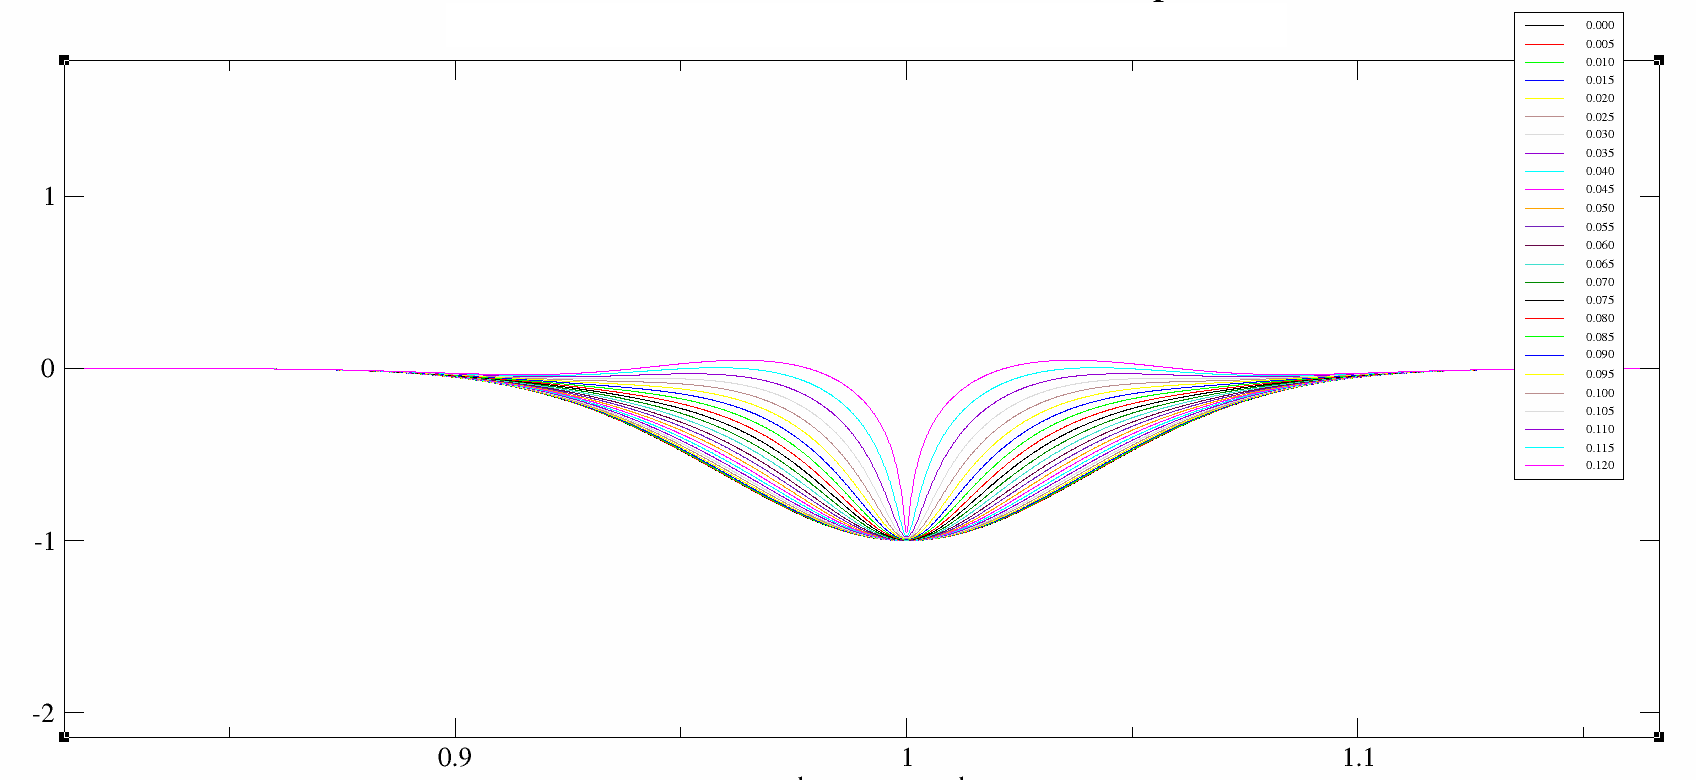
\includegraphics[width=1\textwidth]{peter.png}
  \caption{{\bf{Local divergence}}:The parameters of \eref{eq:main} are $\alpha=5$ and $\beta
    =0.025$ with initial condition
    $u(x,0)=\exp(-30(x-1)^2)$, $u_t(x,0)=0$. (Numerically we take
    periodic boundary conditions.) Note that the second derivative
    diverges in finite time. The simulation corresponds to $\alpha
    /\beta =200$.
  }\label{fig:peter}
\end{figure}


\begin{figure}[h!]
  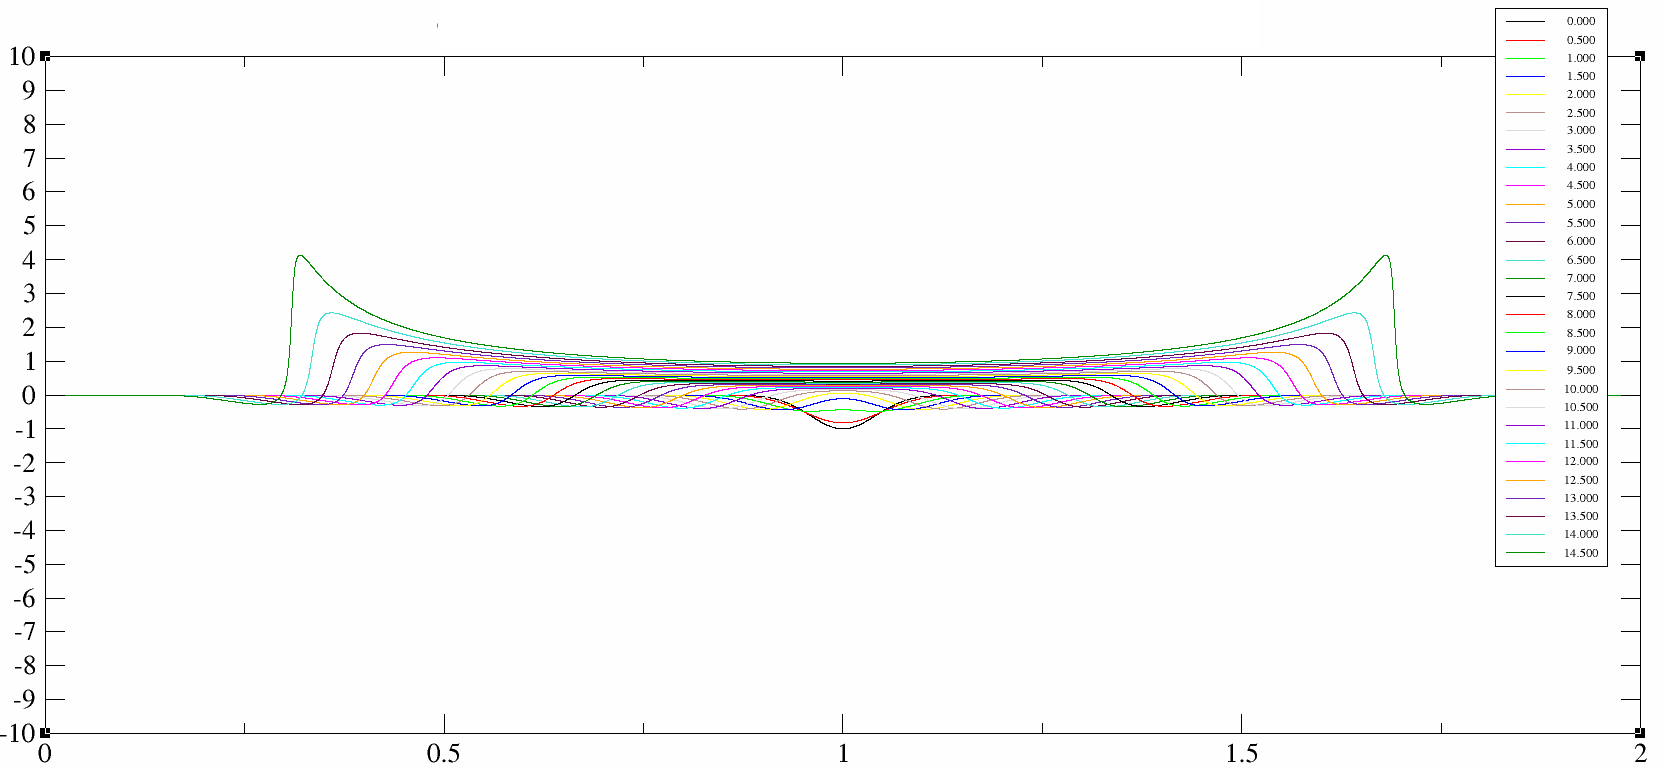
\includegraphics[width=1\textwidth]{divergence.png}
  \caption{{\bf{Wave divergence}}:The nature of divergence ``at infinity.'' As time goes on,
    the support of the function spreads, and the function at the edge
    gets steeper, until the derivative will diverge at some time
    $T_*$.
    The simulation is for the variant equation \eref{eq:main2}, with
    $\alpha=0.01$ and $\beta =0.025$ and initial condition
    $u(x,0)=\exp(-30(x-1)^2)$, $u_x(x,0)=0$. (Numerically we take
    periodic boundary conditions.) Now, $\alpha /\beta =0.4$
  }\label{fig:front}
\end{figure}

We expect that, for fixed $\beta $ a transition between local
divergence and wave divergence will appear. The mathematical situation
for the wave divergence can be explained by an adaptation of the work
of Rammaha \cite{rammaha}. He shows that \eref{eq:main1} will diverge
in finite time under quite weak conditions: \JP{I do this now as if we
  knew the result in dim 1}. 
Take as initial conditions smooth
functions $u(x,0)=f(x)$ and $u_t(x,0)=g(x)$, both with compact support
and assume the support is in $|x|<R$. Fix an $R_0<R$ and define
\begin{equa}
  \epsilon = \frac{1}{2} \int_{x>R_0} (f(x) + (x-R_0) g(x)) \d x~.
\end{equa}
with
\begin{equa}
  M(x)= \frac{1}{2} \left(f(x) + \int_x^R g(\xi)\d\xi\right)>0
\end{equa}
for all $x\in(R_0,R)$.
Then, if $\epsilon >0$ is small enough, Rammaha shows that the
solution must diverge before a time \JP{how does this scale?}
\begin{equa}
  T_* =  \text{ some function of }\epsilon 
\end{equa}

Rammaha's result can be paraphrased as follows. For small initial
The point of the proofs is that {\color{red}(I don't understand this sentence)}, because of the wave character of
\eref{eq:main}, The solution will grow at the advancing front of the
boundary {\color{red}(advancing front of the wave or boundary?)} . And this is shown by a Gronwall-type argument. The
qualitative behavior is clearly seen in \fref{fig:front}.
There are also inequalities which go the other way, Kovalyov
\cite{ehat}, which shows that the solutions live at least as long as {\color{red}(Do you physically understand what does this inequalities tell us practically?)}
\begin{equa}
  T_* \ge  ???? \text{depending on $\epsilon $}
\end{equa}

We will now argue that for $\beta =0$ there are (admittedly unbounded)
initial conditions for which local divergence will appear in
arbitrarily short time. In particular, this time can be shorter than
the wave divergence time.




This divergence is modeled most simply when $\beta =0$. In this case,
taking the (unbounded) initial condition $u(x,0)=A x^2$, 
Eq.\eref{eq:main2} has the explicit solution
  \begin{equa}
    u(x,t)&=\frac{3}{2\alpha (t-t_0)^2}x^2~,\\
  \end{equa}
  when
  \begin{equa}
    u(x,0)&=\frac{3}{2\alpha t_0^2}x^2~,\\
    u_t(x,0)&=\frac{3}{\alpha t_0^3}x^2~.
  \end{equa}
  Clearly, $t_0$ is then just given by {\color{red}(This result is nice and ok, but it does not work when we want to have $u(x,0) = 0$, which is the initial condition that Peter considered. There they showed that the curvature of the minimum blowsup. )}
  \begin{equa}
    t_0=2\frac{u(x,0)}{u_t(x,0)}~.
  \end{equa}
  So we can make $t_0$ arbitrarily short as announced.
Finally, in perturbation theory (up to order $x^4$ included) one can
solve \eref{eq:main1} explicitly (when $\alpha /\beta =1$) in the form
    \begin{equa}
u(x,t)=a(t)\left((x-t)^2+(x+t)^2\right)+b(t) x +c(t)~,
  \end{equa}
  with
  \begin{equa}
    a(t)&=\frac{3}{4A(t-t_0)^2}~,\\
    b(t)&=C_1(t-t_0)^3+C_2\frac{1}{(t-t_0)^2}~,\\
    c(t)&=3\frac{\log(t - t0)}{A} - 3\frac{t_0}{A (t - t0)} -
    3\frac{t0^2}{2A(t - t0)^2} + C_3 t + C_4~.
  \end{equa}
  Therefore, to this order, one can also produce arbitrary rapid local
  divergence, just slightly shifted (by $t_0$) from the origin. {\color{red}(I don't understand the previous argument. The solution does not give us a reasonable behaviour. Because at $t=t_0$ it seems that the logarithm also has problem. )}
\end{document}
